\chapter{Results and Analysis}
\label{ch:resultsAndAnalysis}
\com{
\todo[inline]{
Sometimes this is split into two chapters.\\

Keep in mind: How you are going to evaluate what you have done? What are your metrics?\\
Analysis of your data and proposed solution\\
Does this meet the goals which you had when you started?
}
}

DRAFT

\noindent
In this chapter, we present the results of the localisation and mapping feature added to the \gls{ALM}.


\section{Localisation Analysis}

\noindent Analysis of the Simulated and Outdoor Experiment.

\subsection{Simulated Experiment }
\noindent The extensive and comprehensive experiment run with all the measures available is analysed here.

The following localisation performance have been obtained by the different configurations of sensors.

\begin{figure}[!ht]
	\begin{center}
		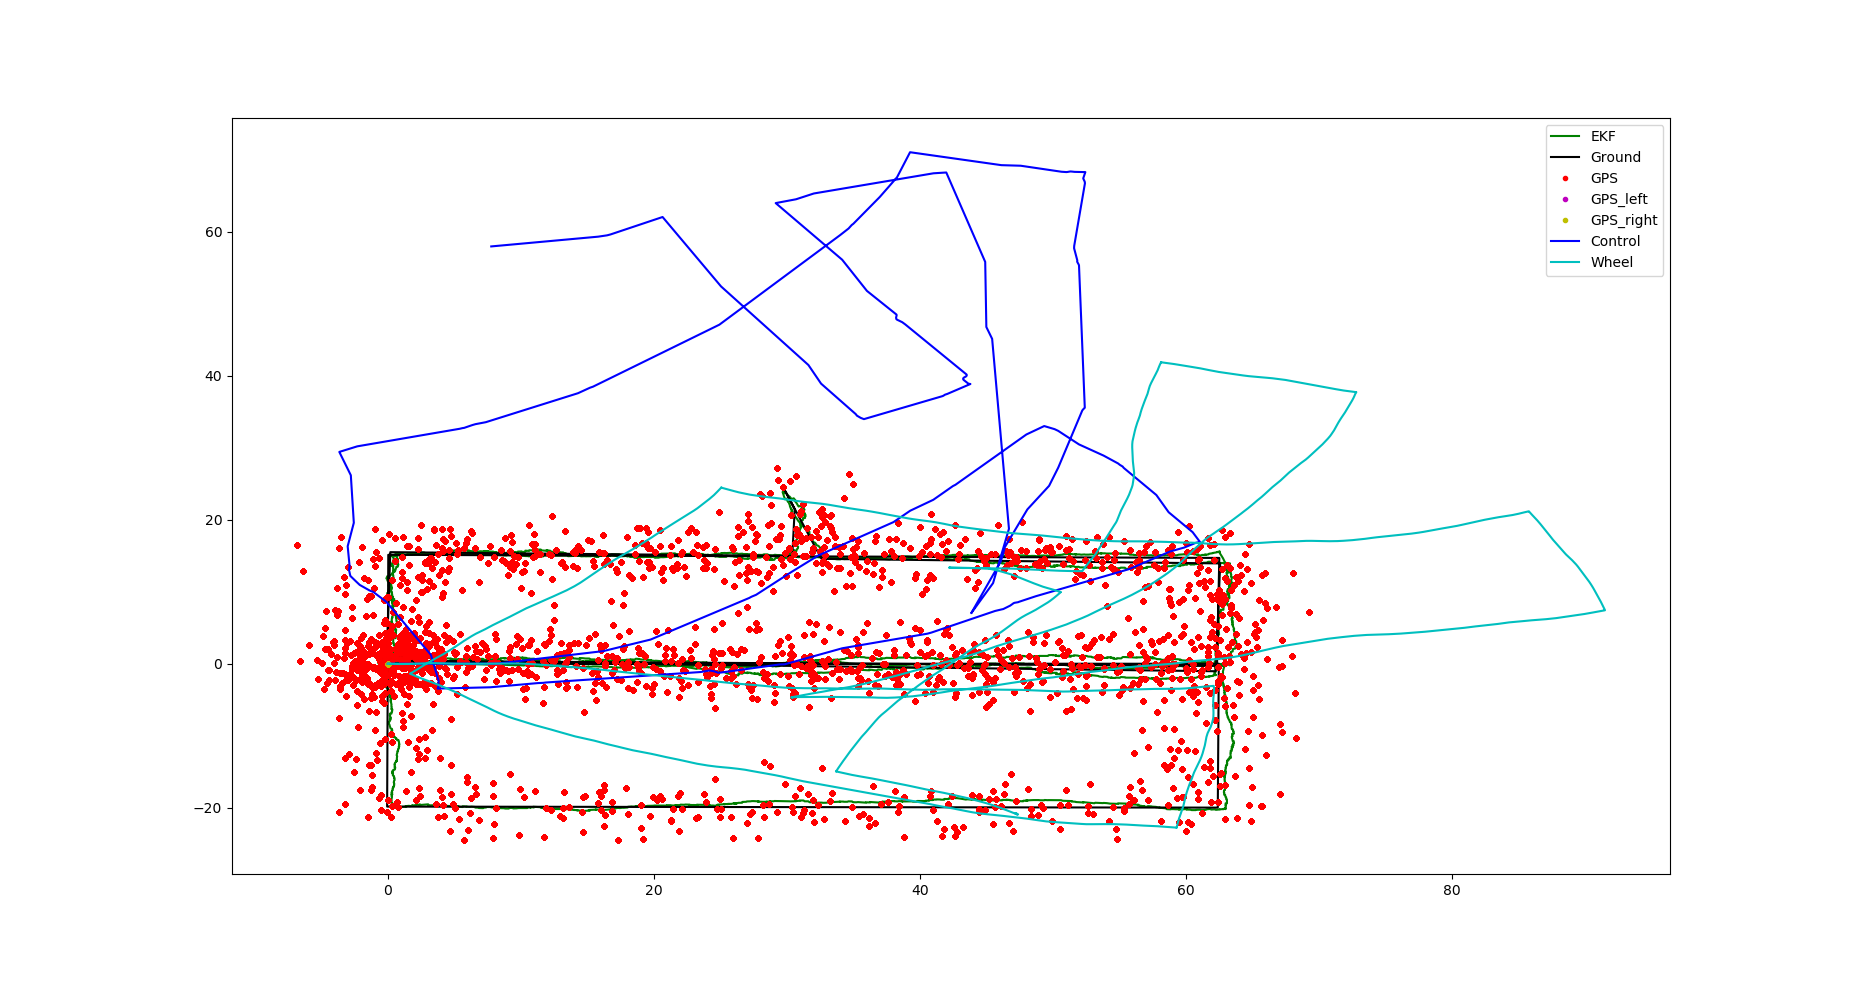
\includegraphics[width=1\textwidth]{Images/5-Results/Sim-Control-WO-GPSs-IMUs.png}
	\end{center}
	\caption{Simulation Experiment Results}
	\label{fig:simRes}
\end{figure}

These results have been evaluated using the \gls{RMSE} metric, the values obtained are showed in the Table below.


	\begin{table}[!ht]
		\small
		\begin{center}
			\label{tab:evalSim}
			\begin{tabular}{|c||S|S|S||S|S|S||S|S|}
				\hline
				\multirow{3}{*}{\textbf{Model}} & \multicolumn{8}{c|}{\textbf{Evaluation}} \\
				& \multicolumn{3}{c||}{\textbf{RMSE}} & \multicolumn{3}{c||}{\textbf{Uncertainty}} & \multicolumn{2}{c|}{\textbf{Time}}\\
				& \multicolumn{1}{c|}{x[m]} & \multicolumn{1}{c|}{y[m]} & \multicolumn{1}{c||}{$\theta$[rad]} & \multicolumn{1}{c|}{x[m]} & \multicolumn{1}{c|}{y[m]} & \multicolumn{1}{c||}{$\theta$[rad]} & \multicolumn{1}{c|}{$\mu$[\SI{}{ms}]} & \multicolumn{1}{c|}{$\sigma$[\SI{}{ms}]}\\
				\hline
				\hline
				\centering{1} & 4.35 & 4.10 & 0.6 & 10.35 & 5.10 & 1.6 & 4.23 & 0.1 \\
				\hline
				\centering{2} & 4.35 & 4.10 & 0.6 & 10.35 & 5.10 & 1.6 & 4.23 & 0.1 \\
				\hline
				\centering{3} & 4.35 & 4.10 & 0.6 & 10.35 & 5.10 & 1.6 & 4.23 & 0.1 \\
				\hline
				\centering{4} & 4.35 & 4.10 & 0.6 & 10.35 & 5.10 & 1.6 & 4.23 & 0.1 \\
				\hline
			\end{tabular}
			\caption{Simulated experiments results}
		\end{center}
	\end{table}


\subsection{Outdoor Experiment }
\noindent The extensive and comprehensive experiments run with all the measures available is analysed here.

The following localisation performance have been obtained by the different configuration of sensors.

\begin{figure}[!ht]
	\begin{center}
		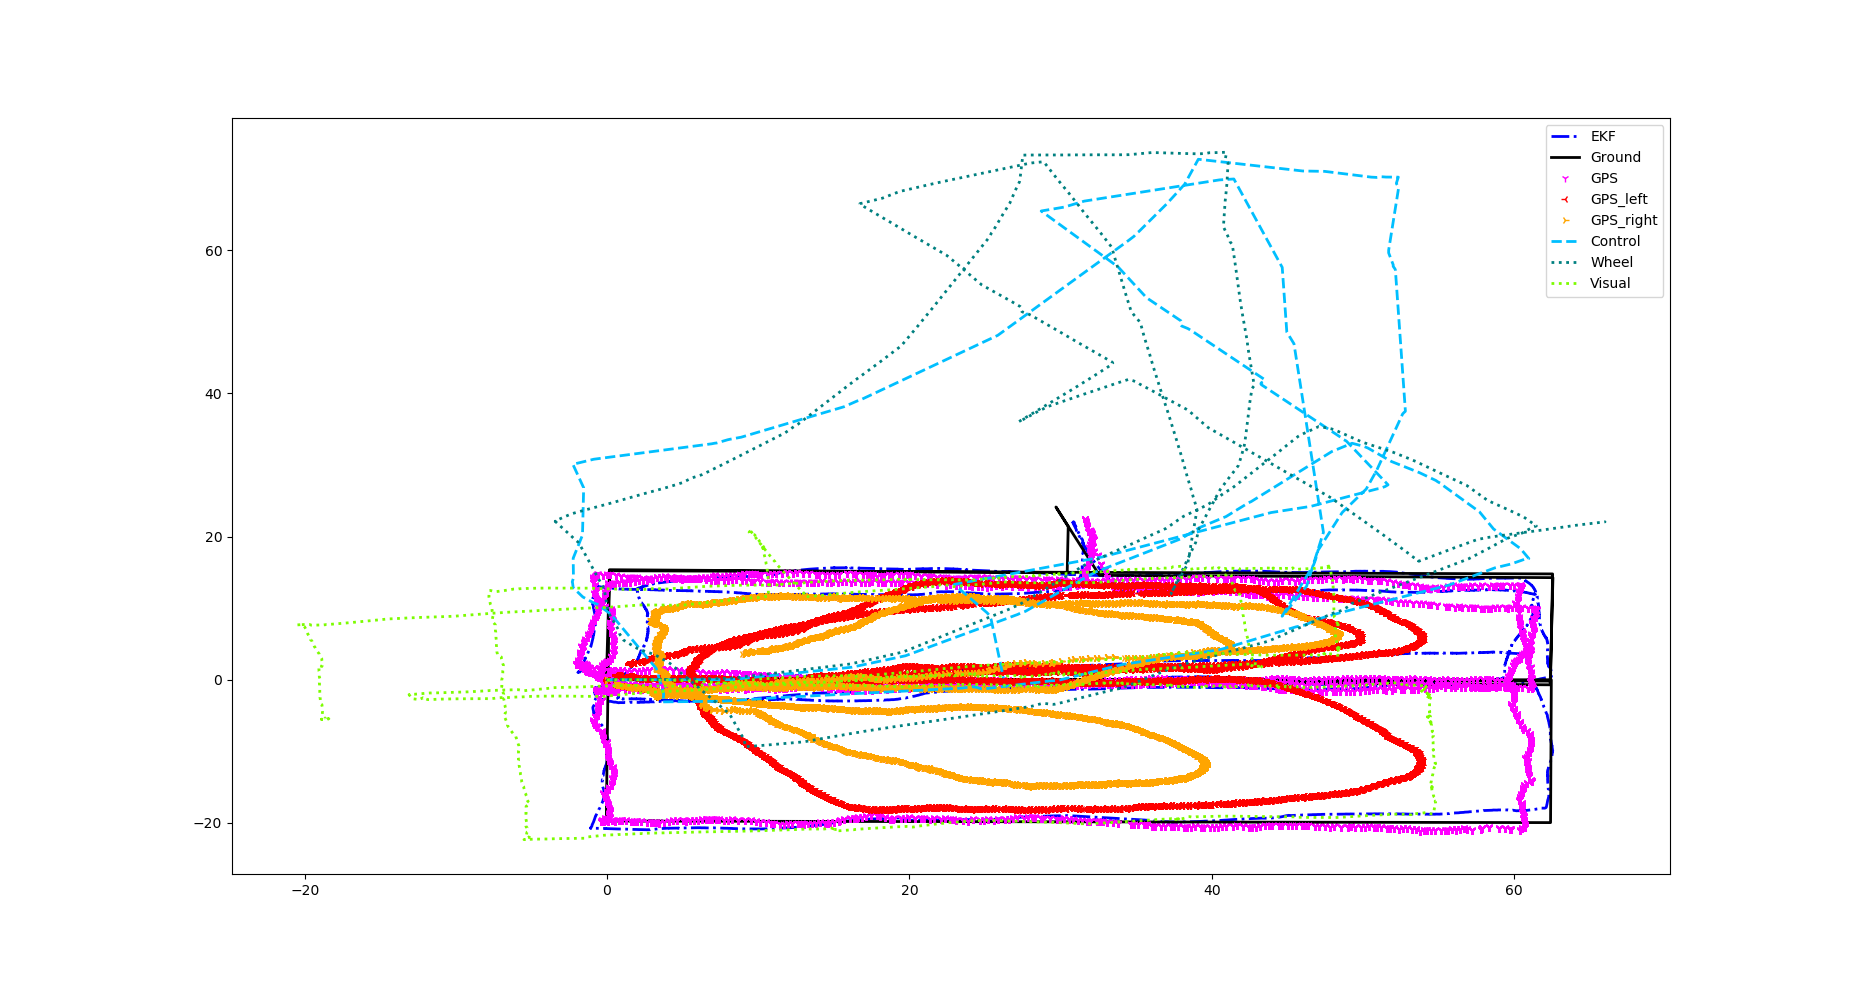
\includegraphics[width=1\textwidth]{Images/5-Results/Out-NoNMEA.png}
	\end{center}
	\caption{Outdoor Experiment Results}
	\label{fig:out}
\end{figure}

These results have been evaluated using the \gls{RMSE} metric, the values obtained are showed in the Table below.


	\begin{table}[!ht]
		\small
		\begin{center}
			\label{tab:evalOutdoor}
			\begin{tabular}{|c||S|S|S||S|S|S||S|S|}
				\hline
				\multirow{3}{*}{\textbf{Model}} & \multicolumn{8}{c|}{\textbf{Evaluation}} \\
				 & \multicolumn{3}{c||}{\textbf{RMSE}} & \multicolumn{3}{c||}{\textbf{Uncertainty}} & \multicolumn{2}{c|}{\textbf{Time}}\\
				 & \multicolumn{1}{c|}{x[m]} & \multicolumn{1}{c|}{y[m]} & \multicolumn{1}{c||}{$\theta$[rad]} & \multicolumn{1}{c|}{x[m]} & \multicolumn{1}{c|}{y[m]} & \multicolumn{1}{c||}{$\theta$[rad]} & \multicolumn{1}{c|}{$\mu$[\SI{}{ms}]} & \multicolumn{1}{c|}{$\sigma$[\SI{}{ms}]}\\
				\hline
				\hline
				\centering{1} & 4.35 & 4.10 & 0.6 & 10.35 & 5.10 & 1.6 & 4.23 & 0.1 \\
				\hline
				\centering{2} & 4.35 & 4.10 & 0.6 & 10.35 & 5.10 & 1.6 & 4.23 & 0.1 \\
				\hline
				\centering{3} & 4.35 & 4.10 & 0.6 & 10.35 & 5.10 & 1.6 & 4.23 & 0.1 \\
				\hline
				\centering{4} & 4.35 & 4.10 & 0.6 & 10.35 & 5.10 & 1.6 & 4.23 & 0.1 \\
				\hline
			\end{tabular}
		\caption{Outdoor experiments results}
		\end{center}
	\end{table}

\section{Mapping Analysis}
\noindent The evolution of the mapping feature is defined here, from the initial setting, to the customised virtual boundary, and finally to the updating map behaviour.


\subsection{Occupancy Grid Boundary}
\noindent
The virtual boundary is then set with the initial run setting of the personalized virtual boundary.
The external area is set to the outdoor limited area.

With this virtual boundary, the automower is able to stay within the designed area.

\begin{figure}[!ht]
	\begin{center}
		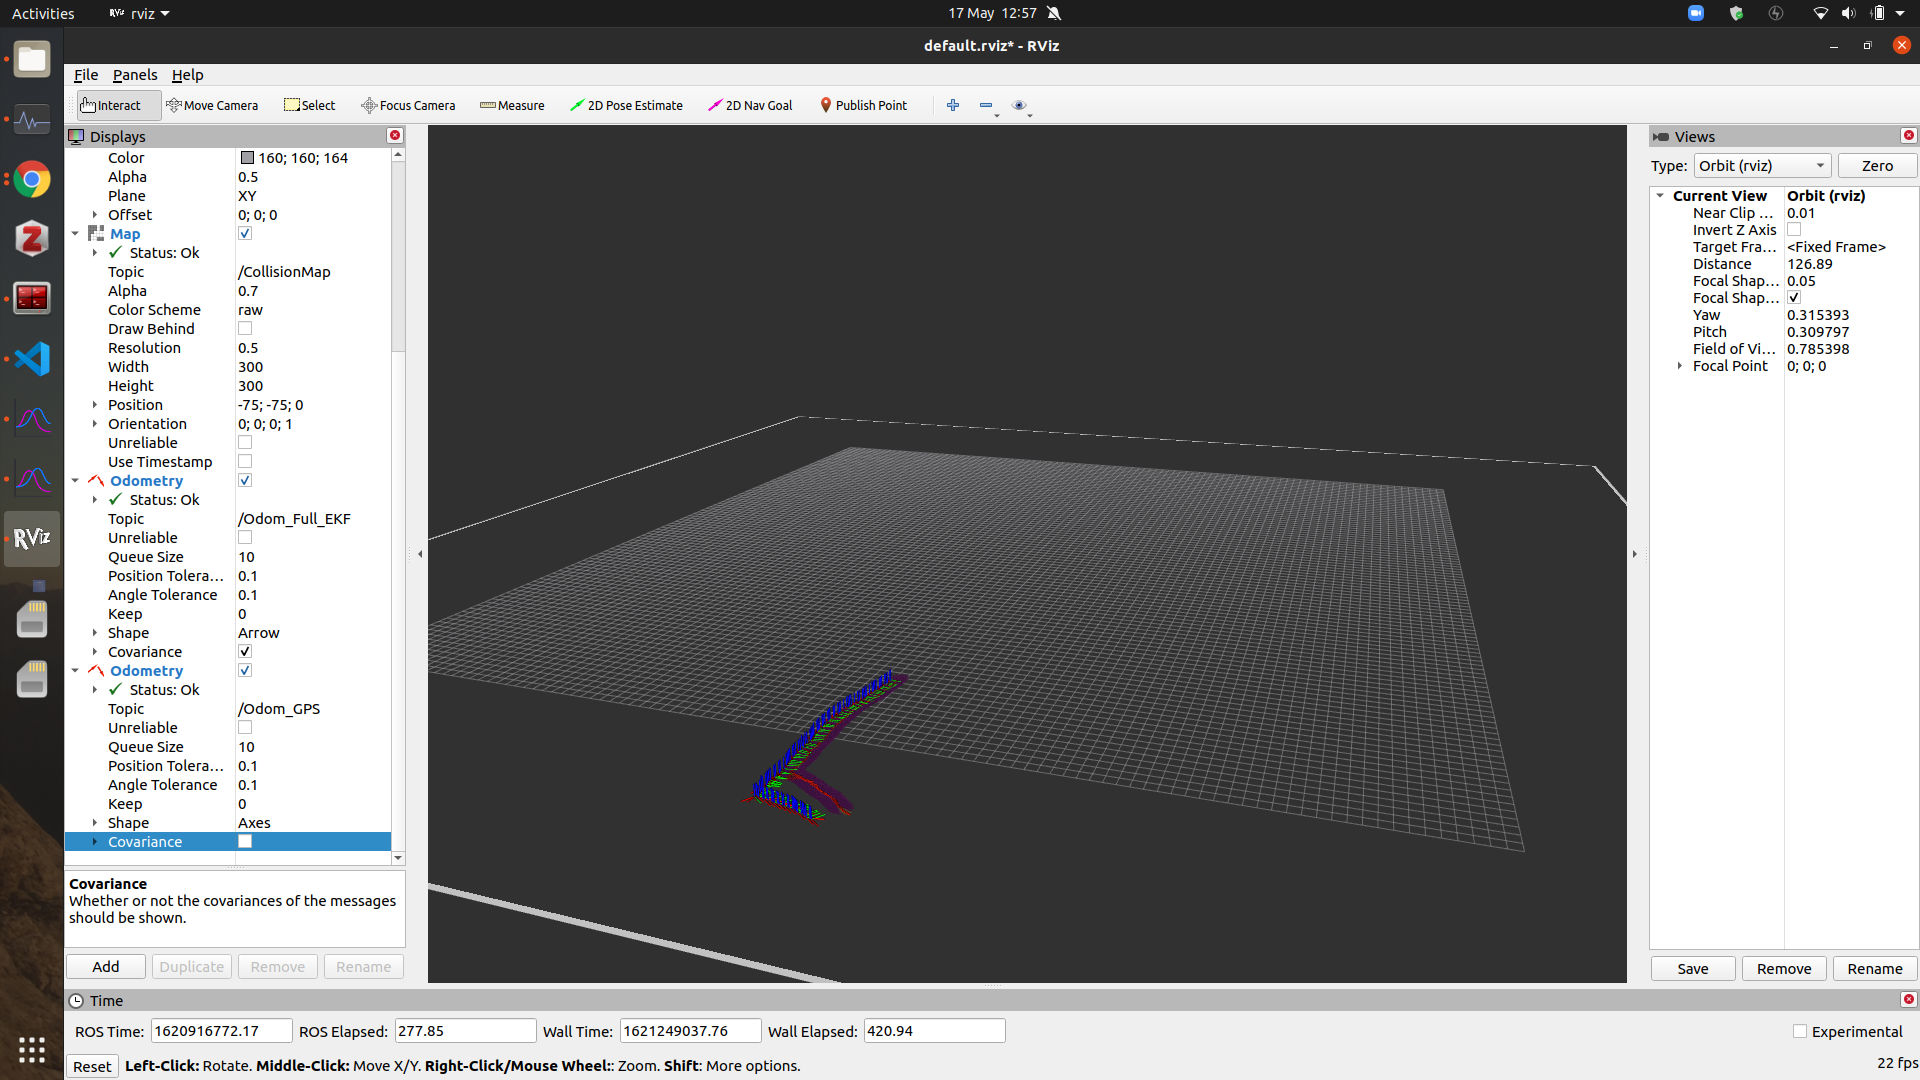
\includegraphics[width=0.75\textwidth]{Images/5-Results/OccupancyGrid.png}
	\end{center}
	\caption{Occupancy Grid Boundary}
	\label{fig:occGridBoud}
\end{figure}


\subsection{Occupancy Grid Update}
\noindent
The virtual boundary is then set with the initial run setting of the personalised virtual boundary.


\begin{figure}[!ht]
	\begin{center}
		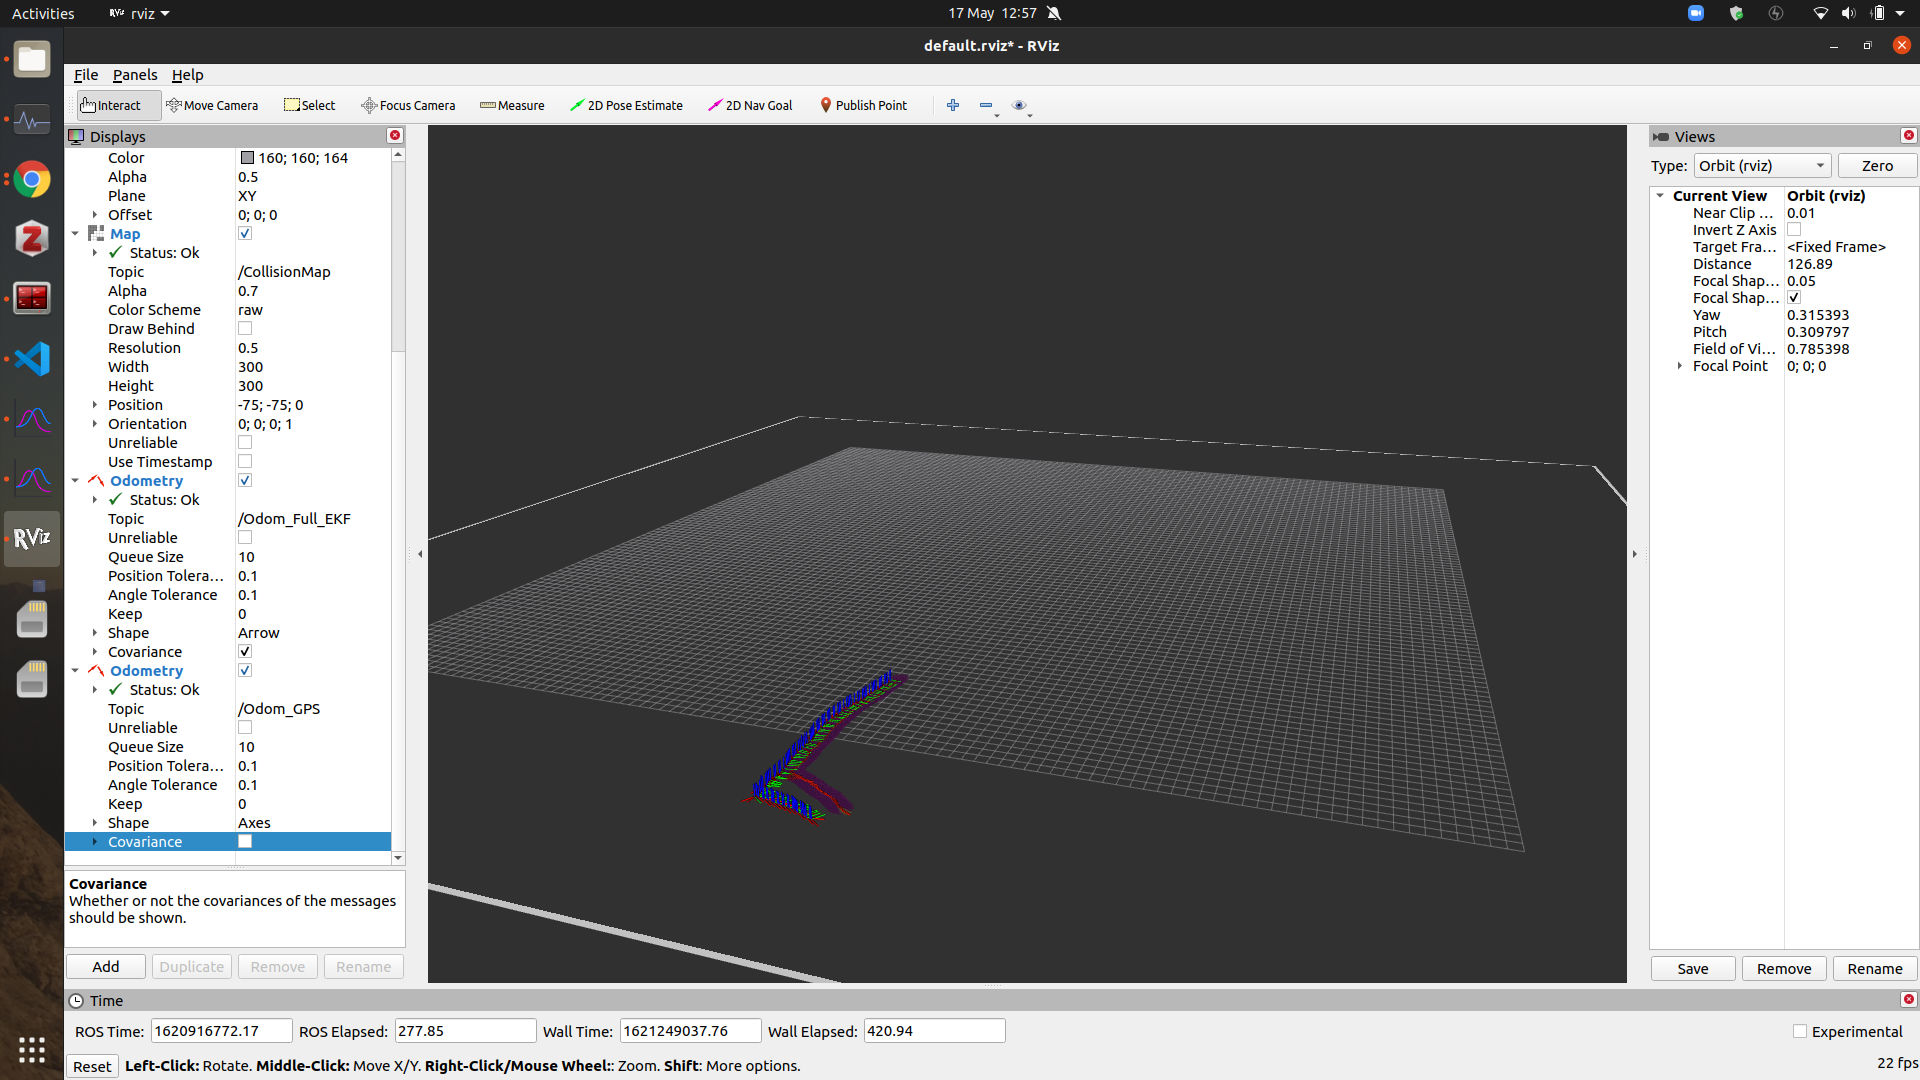
\includegraphics[width=0.75\textwidth]{Images/5-Results/OccupancyGrid.png}
	\end{center}
	\caption{Occupancy Grid Update}
	\label{fig:occGridUpdate}
\end{figure}



%\section{Discussion}

\cleardoublepage
%\clearpage
